\documentclass[aspectratio=43]{beamer}

% Text packages to stop warnings
\usepackage{lmodern}
\usepackage{textcomp}
\usepackage{listings}
\usepackage{multirow}
\usepackage{tikz}

\usetikzlibrary{arrows,automata,shapes,positioning}
\tikzstyle{block} = [rectangle, draw, fill=blue!20, 
    text width=2.5em, text centered, rounded corners, minimum height=2em]
\tikzstyle{bw} = [rectangle, draw, fill=blue!20, 
    text width=3.5em, text centered, rounded corners, minimum height=2em]

% Themes
\usetheme{Boadilla}
\setbeamertemplate{footline}[page number]{}
\setbeamertemplate{navigation symbols}{}

% Suppress the navigation bar
\beamertemplatenavigationsymbolsempty

\lstset{basicstyle=\scriptsize, frame=single}

\newenvironment{changemargin}[1]{% 
  \begin{list}{}{% 
    \setlength{\topsep}{0pt}% 
    \setlength{\leftmargin}{#1}% 
    \setlength{\rightmargin}{1em}
    \setlength{\listparindent}{\parindent}% 
    \setlength{\itemindent}{\parindent}% 
    \setlength{\parsep}{\parskip}% 
  }% 
  \item[]}{\end{list}} 

\title{Lecture 13---Parallelization: Patterns and Strategy}
\subtitle{ECE 459: Programming for Performance}
\date{January 30, 2015}

\begin{document}

%%%%%%%%%%%%%%%%%%%%%%%%%%%%%%%%%%%%%%%%%%%%%%%%%%%%%%%%%%%%%%%%%%%%%%%%%%%%%%%%
\begin{frame}[plain]
  \titlepage
\end{frame}
%%%%%%%%%%%%%%%%%%%%%%%%%%%%%%%%%%%%%%%%%%%%%%%%%%%%%%%%%%%%%%%%%%%%%%%%%%%%%%%%


%%%%%%%%%%%%%%%%%%%%%%%%%%%%%%%%%%%%%%%%%%%%%%%%%%%%%%%%%%%%%%%%%%%%%%%%%%%%%%%%
\begin{frame}
  \frametitle{Assignment 2 Preview}

\large
  \begin{changemargin}{1.5cm}
  Three parts:
  \begin{enumerate}
    \item Restructuring code for Automatic Parallelization.
    \item Manual parallelization of a loop with OpenMP.
    \item Using OpenMP tasks effectively.
  \end{enumerate}

  \end{changemargin}
\end{frame}
%%%%%%%%%%%%%%%%%%%%%%%%%%%%%%%%%%%%%%%%%%%%%%%%%%%%%%%%%%%%%%%%%%%%%%%%%%%%%%%%

\part{More Parallelization Patterns}
\frame{\partpage}

%%%%%%%%%%%%%%%%%%%%%%%%%%%%%%%%%%%%%%%%%%%%%%%%%%%%%%%%%%%%%%%%%%%%%%%%%%%%%%%%
\begin{frame}
  \frametitle{Pattern 5: Pipeline of Tasks}

  \begin{changemargin}{2.5cm}
    Seen briefly in computer architecture.

    \begin{itemize}
    \item Use multiple stages; each thread handles a stage.\\[1em]
     {\bf Example:} a program that handles network packets: (1) accepts
      packets, (2) processes them, and (3) re-transmits them. Could set up the threads such that each packet goes through the threads.
    \vfill
    \item Improves \structure{throughput}; may increase \structure{latency} as
      there's communication between threads.
    \vfill
    \item In the best case, you'll have a linear speedup.\\[1em]

     Rare, since the runtime of the stages will vary, and the slow
      one will be the bottleneck (but you could have 2 instances of the
      slow stage).
  \end{itemize}
  \end{changemargin}
\end{frame}
%%%%%%%%%%%%%%%%%%%%%%%%%%%%%%%%%%%%%%%%%%%%%%%%%%%%%%%%%%%%%%%%%%%%%%%%%%%%%%%%

%%%%%%%%%%%%%%%%%%%%%%%%%%%%%%%%%%%%%%%%%%%%%%%%%%%%%%%%%%%%%%%%%%%%%%%%%%%%%%%%
\begin{frame}
  \frametitle{Pattern 6: Client-Server}

  \begin{changemargin}{2.5cm}
    To execute a large computation, the server supplies work to many
      clients---as many as request it.\\[1em]

    Client computes results and returns them to the server.\\[1em]
   {\bf Examples:} botnets, {\tt SETI@Home}, GUI application (backend
      acts as the server).\\[1em]
   Server can arbitrate access to shared resources (such as network
      access) by storing the requests and sending them out.\\[1em]

   \begin{itemize}
    \item Parallelism is somewhere between single task, multiple threads and
      multiple loosely-coupled tasks  
  \end{itemize}
  \end{changemargin}
\end{frame}
%%%%%%%%%%%%%%%%%%%%%%%%%%%%%%%%%%%%%%%%%%%%%%%%%%%%%%%%%%%%%%%%%%%%%%%%%%%%%%%%

%%%%%%%%%%%%%%%%%%%%%%%%%%%%%%%%%%%%%%%%%%%%%%%%%%%%%%%%%%%%%%%%%%%%%%%%%%%%%%%%
\begin{frame}
  \frametitle{Pattern 7: Producer-Consumer}

  \begin{changemargin}{2.5cm}
    Variant on the pipeline and client-server models.\\
    Producer generates work, and consumer performs work.\\[1em]
    {\bf Example:} producer which generates rendered frames;
      consumer which orders these frames and writes them to disk.\\[1em]
    Any number of producers and consumers.\\[1em]

    \begin{itemize}
    \item This approach can improve \structure{throughput} and also reduces
      design complexity
    \end{itemize}
  \end{changemargin}
\end{frame}
%%%%%%%%%%%%%%%%%%%%%%%%%%%%%%%%%%%%%%%%%%%%%%%%%%%%%%%%%%%%%%%%%%%%%%%%%%%%%%%%

%%%%%%%%%%%%%%%%%%%%%%%%%%%%%%%%%%%%%%%%%%%%%%%%%%%%%%%%%%%%%%%%%%%%%%%%%%%%%%%%
\begin{frame}
  \frametitle{Combining Strategies}

  \begin{changemargin}{2.5cm}
    Most problems don't fit into one category, so it's often best to combine
      strategies.\\[1em]

    For instance, you might often start with a pipeline, and then use
      multiple threads in a particular pipeline stage to handle one piece of
      data.\\[1em]
    Tip: estimate to see what divisions of strategies would work best
      (might have to do more iterations of Amdahl's law depending on the amount
      of strategies you can use).
  \end{changemargin}

\end{frame}
%%%%%%%%%%%%%%%%%%%%%%%%%%%%%%%%%%%%%%%%%%%%%%%%%%%%%%%%%%%%%%%%%%%%%%%%%%%%%%%%

%%%%%%%%%%%%%%%%%%%%%%%%%%%%%%%%%%%%%%%%%%%%%%%%%%%%%%%%%%%%%%%%%%%%%%%%%%%%%%%%
\begin{frame}
  \frametitle{Midterm Questions from 2011 (1)}

\begin{changemargin}{2.5cm}
  For each of the following situations, {\bf name an appropriate parallelization
  pattern and the granularity at which you would apply it, explain the necessary
  communication, and explain why your pattern is appropriate}.
  \begin{itemize}
  \item build system, e.g. parallel make
    \begin{itemize}
      \item<2-> Multiple independent tasks, at a per-file granularity
    \end{itemize}
  \item optical character recognition system
    \begin{itemize}
      \item<2-> Pipeline of tasks
      \item<2-> 2 tasks - finding characters and analyzing them
    \end{itemize}
  \end{itemize}
\end{changemargin}
\end{frame}
%%%%%%%%%%%%%%%%%%%%%%%%%%%%%%%%%%%%%%%%%%%%%%%%%%%%%%%%%%%%%%%%%%%%%%%%%%%%%%%%

%%%%%%%%%%%%%%%%%%%%%%%%%%%%%%%%%%%%%%%%%%%%%%%%%%%%%%%%%%%%%%%%%%%%%%%%%%%%%%%%
\begin{frame}
  \frametitle{Midterm Questions from 2011 (2)}

\begin{changemargin}{2.5cm}
  {\bf Give a concrete example} where you would use the following
  parallelization patterns. {\bf Explain} the granularity at which you'd apply
  the pattern.
  \begin{itemize}
    \item single task, multiple threads:
    \begin{itemize}
      \item<2-> Computation of a mathematical function with independent
        sub-formulas.
    \end{itemize}
    \item producer-consumer (no rendering frames, please):
    \begin{itemize}
      \item<2-> Processing of stock-market data:
        a server might generate raw financial data (quotes) for a
        particular security. The server would be the producer. Several clients
        (or consumers) may take the raw data and use them in different ways, e.g. by computing means, generating charts, etc.
    \end{itemize}
  \end{itemize}
 \end{changemargin}
\end{frame}
%%%%%%%%%%%%%%%%%%%%%%%%%%%%%%%%%%%%%%%%%%%%%%%%%%%%%%%%%%%%%%%%%%%%%%%%%%%%%%%%

%%%%%%%%%%%%%%%%%%%%%%%%%%%%%%%%%%%%%%%%%%%%%%%%%%%%%%%%%%%%%%%%%%%%%%%%%%%%%%%%
\part{Parallelizing Code}
\frame{\partpage}

%%%%%%%%%%%%%%%%%%%%%%%%%%%%%%%%%%%%%%%%%%%%%%%%%%%%%%%%%%%%%%%%%%%%%%%%%%%%%%%%
\begin{frame}
  \frametitle{How To Parallelize Code: Strategy}
  
  \begin{changemargin}{2.5cm}
  Four-step outline:
  \begin{enumerate}
    \item Profile the code.
    \item Look at hotspots; find and optimize dependencies; parallelize dependency chains; change the algorithm if you can.
    \item Estimate benefits.
    \item If not good enough, step back and try higher level of abstraction.
  \end{enumerate}
  Always try to minimize synchronization.
  \end{changemargin}

\end{frame}
%%%%%%%%%%%%%%%%%%%%%%%%%%%%%%%%%%%%%%%%%%%%%%%%%%%%%%%%%%%%%%%%%%%%%%%%%%%%%%%%


%%%%%%%%%%%%%%%%%%%%%%%%%%%%%%%%%%%%%%%%%%%%%%%%%%%%%%%%%%%%%%%%%%%%%%%%%%%%%%%%
\begin{frame}
  \frametitle{Low-level Implementation Tactic: Thread Pools}
  
  \begin{changemargin}{2.5cm}
    Instead of creating threads, destroying them and recreating them, you
      can use a \structure{thread pool}.
    \begin{itemize}
    \item It creates $n$ threads; you just {\tt push} work onto them.
    \end{itemize}

  \begin{center}
    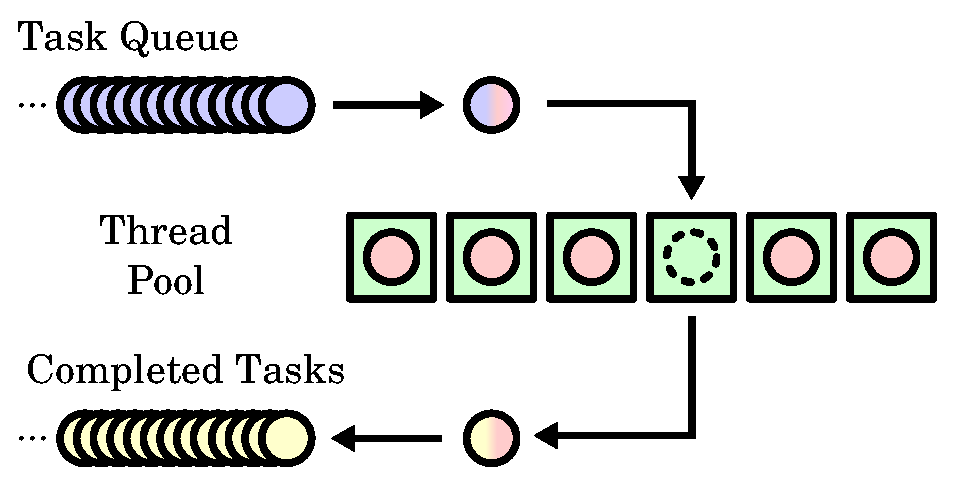
\includegraphics[scale=0.4]{L13/thread-pool}
  \end{center}

  \begin{itemize}
    \item Only question is: How many threads should you create? (Experiment to find out).
    \item Implementation from GLib: {\tt GThreadPool}.
  \end{itemize}
  \end{changemargin}

\end{frame}
%%%%%%%%%%%%%%%%%%%%%%%%%%%%%%%%%%%%%%%%%%%%%%%%%%%%%%%%%%%%%%%%%%%%%%%%%%%%%%%%


%%%%%%%%%%%%%%%%%%%%%%%%%%%%%%%%%%%%%%%%%%%%%%%%%%%%%%%%%%%%%%%%%%%%%%%%%%%%%%%%
\begin{frame}
  \frametitle{Introduction to Automatic Parallelization}

  \begin{changemargin}{2.5cm}
    Vision: take a sequential C program and \\ automatically convert it into a parallel version.\\[1em]

    Lots of research in the early 1990s, then tapered off.\\~~~(it's hard!)\\[1em]

    Renewed interest now since multicores are so common.\\~~~(it's still hard!)
  \end{changemargin}
\end{frame}
%%%%%%%%%%%%%%%%%%%%%%%%%%%%%%%%%%%%%%%%%%%%%%%%%%%%%%%%%%%%%%%%%%%%%%%%%%%%%%%%

%%%%%%%%%%%%%%%%%%%%%%%%%%%%%%%%%%%%%%%%%%%%%%%%%%%%%%%%%%%%%%%%%%%%%%%%%%%%%%%%
\begin{frame}
  \frametitle{What Can We Parallelize?}

  \begin{changemargin}{2.5cm}
  
  \begin{itemize}
    \item Some languages are easier than others to reason about (and therefore to
      automatically parallelize).
    \item C can be easy to parallelize, given the right code, plus compiler hints.
    \item ``The right code'' = arrays with no loop-carried dependencies.
  \end{itemize}
  \end{changemargin}
\end{frame}

%%%%%%%%%%%%%%%%%%%%%%%%%%%%%%%%%%%%%%%%%%%%%%%%%%%%%%%%%%%%%%%%%%%%%%%%%%%%%%%%
\begin{frame}
  \frametitle{Automatic Parallelization in Practice}
  \begin{changemargin}{2cm}
    Some production compilers support automatic parallelization: 
    \begin{itemize}
      \item {\tt icc} (Intel's
      non-free compiler);
      \item {\tt solarisstudio} (Oracle's free-as-in-beer
      compiler \footnote{\tiny \url{http://www.oracle.com/technetwork/documentation/solaris-studio-12-192994.html}});
      \item {\tt gcc} (GNU's free-as-in-speech compiler).
    \end{itemize}
  \end{changemargin}

\end{frame}
%%%%%%%%%%%%%%%%%%%%%%%%%%%%%%%%%%%%%%%%%%%%%%%%%%%%%%%%%%%%%%%%%%%%%%%%%%%%%%%%

%%%%%%%%%%%%%%%%%%%%%%%%%%%%%%%%%%%%%%%%%%%%%%%%%%%%%%%%%%%%%%%%%%%%%%%%%%%%%%%%
\begin{frame}[fragile]
  \frametitle{Example Code from the Textbook}

  \begin{changemargin}{1.5cm}
    We saw automatic parallelization of some code.\\
    Let's revisit the whole issue in Lecture 15.
  \end{changemargin}
  
\end{frame}
%%%%%%%%%%%%%%%%%%%%%%%%%%%%%%%%%%%%%%%%%%%%%%%%%%%%%%%%%%%%%%%%%%%%%%%%%%%%%%%%

%%%%%%%%%%%%%%%%%%%%%%%%%%%%%%%%%%%%%%%%%%%%%%%%%%%%%%%%%%%%%%%%%%%%%%%%%%%%%%%%
\part{Parallelizing Code}
\frame{\partpage}

%%%%%%%%%%%%%%%%%%%%%%%%%%%%%%%%%%%%%%%%%%%%%%%%%%%%%%%%%%%%%%%%%%%%%%%%%%%%%%%%
\begin{frame}[fragile]
  \frametitle{Example Code from the Textbook}

\begin{changemargin}{1.5cm}
Following Gove, we'll parallelize the following code:

  \begin{lstlisting}[numbers=left]
#include <stdlib.h>

void setup(double *vector, int length) {
    int i;
    for (i = 0; i < length; i++)
    {
        vector[i] += 1.0;
    }
}

int main()
{
    double *vector;
    vector = (double*) malloc(sizeof(double)*1024*1024);
    for (int i = 0; i < 1000; i++)
    {
        setup (vector, 1024*1024);
    }
}
  \end{lstlisting}
\end{changemargin}
\end{frame}
%%%%%%%%%%%%%%%%%%%%%%%%%%%%%%%%%%%%%%%%%%%%%%%%%%%%%%%%%%%%%%%%%%%%%%%%%%%%%%%%

%%%%%%%%%%%%%%%%%%%%%%%%%%%%%%%%%%%%%%%%%%%%%%%%%%%%%%%%%%%%%%%%%%%%%%%%%%%%%%%%
\begin{frame}[fragile]
  \frametitle{Automatic Parallelization of Example Code}

\begin{changemargin}{1.5cm}
  Let's try automatic parallelization.
  \vfill
  Compiling with {\tt solarisstudio} and automatic parallelization yields
  the following:
\end{changemargin}

{\scriptsize
  \begin{lstlisting}
% solarisstudio-cc -O3 -xautopar -xloopinfo omp_vector.c 
"omp_vector.c", line 5: PARALLELIZED, and serial version generated                 
"omp_vector.c", line 15: not parallelized, call may be unsafe
  \end{lstlisting}
}
\begin{changemargin}{1.5cm}
  How will this code compare to our manual efforts? \\
  (If you weren't in class, you'll have to try it yourself.)
  \vfill
  {\bf Note:} {\tt solarisstudio} generates two versions of the code, 
  and decides, at runtime, if the parallel code would be faster.
\end{changemargin}

\end{frame}
%%%%%%%%%%%%%%%%%%%%%%%%%%%%%%%%%%%%%%%%%%%%%%%%%%%%%%%%%%%%%%%%%%%%%%%%%%%%%%%%

%%%%%%%%%%%%%%%%%%%%%%%%%%%%%%%%%%%%%%%%%%%%%%%%%%%%%%%%%%%%%%%%%%%%%%%%%%%%%%%%
\begin{frame}[fragile]
  \frametitle{Autoparallelization implementation: OpenMP}

\begin{changemargin}{1.5cm}
  Under the hood, most parallelization frameworks use {\tt OpenMP},
      which we'll see next lecture.\\[1em]
  For now: you can control the number of threads with the
      {\tt OMP\_NUM\_THREADS} environment variable.\\[1em]
\end{changemargin}
\end{frame}
%%%%%%%%%%%%%%%%%%%%%%%%%%%%%%%%%%%%%%%%%%%%%%%%%%%%%%%%%%%%%%%%%%%%%%%%%%%%%%%%

%%%%%%%%%%%%%%%%%%%%%%%%%%%%%%%%%%%%%%%%%%%%%%%%%%%%%%%%%%%%%%%%%%%%%%%%%%%%%%%%
\begin{frame}[fragile]
  \frametitle{Automatic Parallelization in {\tt gcc}}

\begin{changemargin}{1.5cm}
  {\tt gcc} (since 4.3) can also auto-parallelize loops. \\
  However, there are
      a few problems:
      \begin{enumerate}
        \item It will not tell you which loops it parallelizes (nicely).
        \item It only operates with a fixed number of threads.
        \item The profitability metrics are quite simple.
        \item Only operates in simple cases.
      \end{enumerate}
   ~\\[1em]

  Use the flag {\tt -ftree-parallelize-loops=N} where {\tt N} is the number of
  threads.
  \vfill
  {\bf Note:} {\tt gcc} also uses {\tt OpenMP} but ignores
  {\tt OMP\_NUM\_THREADS}.
\end{changemargin}

\end{frame}
%%%%%%%%%%%%%%%%%%%%%%%%%%%%%%%%%%%%%%%%%%%%%%%%%%%%%%%%%%%%%%%%%%%%%%%%%%%%%%%%

%%%%%%%%%%%%%%%%%%%%%%%%%%%%%%%%%%%%%%%%%%%%%%%%%%%%%%%%%%%%%%%%%%%%%%%%%%%%%%%%
\begin{frame}[fragile]
  \frametitle{Understanding Automatic Parallelization in {\tt gcc}}

\begin{changemargin}{1.5cm}
  Flag {\tt -fdump-tree-parloops-details} shows what the automatic
  parallelizations were, but it's quite unreadable.
  \vfill
  Instead, you can look at the assembly code to see the parallelizations
  (obviously, impractical for a large project).
  \begin{lstlisting}
% gcc -std=c99 -O3 -ftree-parallelize-loops=4
  omp_vector_gcc.c -S -o omp_vector_gcc_auto.s
  \end{lstlisting}
  \vfill
  The resulting {\tt .s} file contains the following code:
  \begin{lstlisting}
call    GOMP_parallel_start
leaq    80(%rsp), %rdi
call    setup._loopfn.0
call    GOMP_parallel_end
  \end{lstlisting}
  \vfill
  {\bf Note:} {\tt gcc} also parallelizes {\tt main.\_loopfn.2} and
  {\tt main.\_loopfn.3}, although it looks like it serves little purpose.
\end{changemargin}

\end{frame}
%%%%%%%%%%%%%%%%%%%%%%%%%%%%%%%%%%%%%%%%%%%%%%%%%%%%%%%%%%%%%%%%%%%%%%%%%%%%%%%%

%%%%%%%%%%%%%%%%%%%%%%%%%%%%%%%%%%%%%%%%%%%%%%%%%%%%%%%%%%%%%%%%%%%%%%%%%%%%%%%%
\begin{frame}
  \frametitle{Manually Parallelizing the Example Code}

\begin{changemargin}{1.5cm}
  What can we do to parallelize this code?
  \vfill
  {\bf Option 1:} \uncover<2->{ horizontal~ \qquad \begin{minipage}{7em} --- --- --- ---\\[-.8em] --- --- --- ---\\[-.8em] --- --- --- --- \end{minipage}}

  \begin{itemize}
    \item<2-> Create 4 threads; each thread does 1000 iterations on its own sub-array.
  \end{itemize}

  {\bf Option 2:} \uncover<3->{ bad horizontal~~ \begin{minipage}{7em} --- --- --- ---\\[-.8em] --- --- --- ---\\[-.8em] --- --- --- --- \end{minipage}}

  \begin{itemize}
    \item<3-> 1000 times, create 4 threads which each operate once on the sub-array.
  \end{itemize}

  {\bf Option 3:} \uncover<4->{~~vertical $ \quad \: \qquad \mid \mid \mid\mid \:\: \mid \mid \mid \mid \:\: \mid \mid \mid \mid\:\: \mid \mid \mid \mid$}
  \begin{itemize}
    \item<4-> Create 4 threads; for each element, the owning thread does 1000 iterations on that element.
  \end{itemize}
\end{changemargin}
\end{frame}
%%%%%%%%%%%%%%%%%%%%%%%%%%%%%%%%%%%%%%%%%%%%%%%%%%%%%%%%%%%%%%%%%%%%%%%%%%%%%%%%

%%%%%%%%%%%%%%%%%%%%%%%%%%%%%%%%%%%%%%%%%%%%%%%%%%%%%%%%%%%%%%%%%%%%%%%%%%%%%%%%
\begin{frame}
  \frametitle{Manual Parallelization Demo}

\begin{changemargin}{1.5cm}
  I'll show a demo of three example PThread parallelizations.\\[1em]

  Methodology: compiling with {\tt solarisstudio}, \\ flags {\tt -O3 -lpthread}.\\[1em]

  Which manual option performs better?
\end{changemargin}

\end{frame}
%%%%%%%%%%%%%%%%%%%%%%%%%%%%%%%%%%%%%%%%%%%%%%%%%%%%%%%%%%%%%%%%%%%%%%%%%%%%%%%%


%%%%%%%%%%%%%%%%%%%%%%%%%%%%%%%%%%%%%%%%%%%%%%%%%%%%%%%%%%%%%%%%%%%%%%%%%%%%%%%%
\begin{frame}[fragile]
  \frametitle{Comparing Parallelization Results}

\begin{changemargin}{1.5cm}
How does autoparallelization compare to manual parallelization?
  %% \begin{itemize}
  %%   \item<2-> Relative ordering: {\bf Option 3} \textgreater{} Automatic
  %%     \textgreater{} {\bf Option 1}
  %%   \item<2-> Automatic parallelization of {\bf Option 1} was better than
  %%     manual, why?
  %%   \item<3-> Manual {\bf Option 3} performed better, even though both used the
  %%     same number of threads, why?
  %% \end{itemize}
\end{changemargin}

\end{frame}
%%%%%%%%%%%%%%%%%%%%%%%%%%%%%%%%%%%%%%%%%%%%%%%%%%%%%%%%%%%%%%%%%%%%%%%%%%%%%%%%



%%%%%%%%%%%%%%%%%%%%%%%%%%%%%%%%%%%%%%%%%%%%%%%%%%%%%%%%%%%%%%%%%%%%%%%%%%%%%%%%
\begin{frame}[fragile]
  \frametitle{Case Study 2: Multiplying a Matrix by a Vector}

\begin{changemargin}{1.5cm}
Let's see how automatic parallelization does on a more complicated
program (could we parallelize this?):

  \begin{lstlisting}[numbers=left]
void matVec (double **mat, double *vec, double *out,
             int *row, int *col) 
{
  int i, j;
  for (i = 0; i < *row; i++)
  {
    out[i] = 0;
    for (j = 0; j < *col; j++)
    {
      out[i] += mat[i][j] * vec[j];
    }
  }
}
  \end{lstlisting}
\end{changemargin}

  \begin{center}
    Reminder:
    \begin{math}
      \begin{bmatrix} 1 & 2 & 3 \\ 4 & 5 & 6\end{bmatrix}
      \begin{bmatrix} 1 \\ 2 \\ 3 \end{bmatrix}
      =
      \begin{bmatrix} 14 \\ 32 \end{bmatrix}
    \end{math}
  \end{center}

\end{frame}
%%%%%%%%%%%%%%%%%%%%%%%%%%%%%%%%%%%%%%%%%%%%%%%%%%%%%%%%%%%%%%%%%%%%%%%%%%%%%%%%

%%%%%%%%%%%%%%%%%%%%%%%%%%%%%%%%%%%%%%%%%%%%%%%%%%%%%%%%%%%%%%%%%%%%%%%%%%%%%%%%
\begin{frame}[fragile]
  \frametitle{Case Study: Automatic Parallelization, Attempt 1}

  \begin{changemargin}{2.5cm}
  Well, based on our knowledge, we could parallelize the outer loop.\\[1em]
  Let's see what {\tt solarisstudio} will do for us\ldots
  \end{changemargin}

  \begin{lstlisting}
% solarisstudio-cc -xautopar -xloopinfo -O3 -c fploop.c
"fploop.c", line 5: not parallelized, not a recognized for loop
"fploop.c", line 8: not parallelized, not a recognized for loop
  \end{lstlisting}

  \begin{changemargin}{2.5cm}
  \ldots it refuses to do anything, guesses?
  \end{changemargin}

\end{frame}
%%%%%%%%%%%%%%%%%%%%%%%%%%%%%%%%%%%%%%%%%%%%%%%%%%%%%%%%%%%%%%%%%%%%%%%%%%%%%%%%

%%%%%%%%%%%%%%%%%%%%%%%%%%%%%%%%%%%%%%%%%%%%%%%%%%%%%%%%%%%%%%%%%%%%%%%%%%%%%%%%
\begin{frame}[fragile]
  \frametitle{Case Study: Automatic Parallelization, Attempt 2}

\begin{changemargin}{1cm}
  \begin{itemize}
    \item The loop bounds are not constant, since one of the variables may alias
      {\tt row} or {\tt col}, even though {\tt int $\neq$ double}.
  \end{itemize}
~\\[1em]

  So, let's add {\tt restrict} to {\tt row} and {\tt col} and see what
  happens\ldots

  \begin{lstlisting}
% solarisstudio-cc -O3 -xautopar -xloopinfo -c fploop.c
"fploop.c", line 5: not parallelized, unsafe dependence
"fploop.c", line 8: not parallelized, unsafe dependence
  \end{lstlisting}

  Now it recognizes the loop, but still won't parallelize it. Why?
\end{changemargin}

\end{frame}
%%%%%%%%%%%%%%%%%%%%%%%%%%%%%%%%%%%%%%%%%%%%%%%%%%%%%%%%%%%%%%%%%%%%%%%%%%%%%%%%

%%%%%%%%%%%%%%%%%%%%%%%%%%%%%%%%%%%%%%%%%%%%%%%%%%%%%%%%%%%%%%%%%%%%%%%%%%%%%%%%
\begin{frame}[fragile]
  \frametitle{Case Study: Automatic Parallelization, Attempt 3}

\begin{changemargin}{1cm}
  \begin{itemize}
    \item {\tt out} might alias {\tt mat} or {\tt vec}, which would make this
      unsafe
  \end{itemize}

  Let's add another {\tt restrict} to {\tt out}:

  \begin{lstlisting}
% solarisstudio-cc -O3 -xautopar -xloopinfo -c fploop.c
"fploop.c", line 5: PARALLELIZED, and serial version
  generated
"fploop.c", line 8: not parallelized, unsafe dependence
  \end{lstlisting}

  Now, we can get the outer loop to parallelize.
  
  \begin{itemize}
    \item Parallelizing the outer loop is almost always better than inner loops,
      and usually it's a waste to do both, so we're done.
  \end{itemize}

  {\bf Note:} We can parallelize the inner loop as well (it's similar to
  Assignment 1). We'll see that {\tt solarisstudio} can do it automatically.
\end{changemargin}

\end{frame}
%%%%%%%%%%%%%%%%%%%%%%%%%%%%%%%%%%%%%%%%%%%%%%%%%%%%%%%%%%%%%%%%%%%%%%%%%%%%%%%%

%%%%%%%%%%%%%%%%%%%%%%%%%%%%%%%%%%%%%%%%%%%%%%%%%%%%%%%%%%%%%%%%%%%%%%%%%%%%%%%%
\begin{frame}[fragile]
  \frametitle{Loops That gcc's Automatic Parallelization Can Handle}

\begin{changemargin}{2.5cm}
  Single loop:
  \begin{lstlisting}
for (i = 0; i < 1000; i++)
    x[i] = i + 3;
  \end{lstlisting}
  \vfill
  Nested loops with simple dependency:
  \begin{lstlisting}
for (i = 0; i < 100; i++)
    for (j = 0; j < 100; j++)
        X[i][j] = X[i][j] + Y[i-1][j];
  \end{lstlisting}
  \vfill
  Single loop with not-very-simple dependency:
  \begin{lstlisting}
for (i = 0; i < 10; i++)
    X[2*i+1] = X[2*i];
  \end{lstlisting}
\end{changemargin}
\end{frame}
%%%%%%%%%%%%%%%%%%%%%%%%%%%%%%%%%%%%%%%%%%%%%%%%%%%%%%%%%%%%%%%%%%%%%%%%%%%%%%%%

%%%%%%%%%%%%%%%%%%%%%%%%%%%%%%%%%%%%%%%%%%%%%%%%%%%%%%%%%%%%%%%%%%%%%%%%%%%%%%%%
\begin{frame}[fragile]
  \frametitle{Loops That gcc's Automatic Parallelization Can't Handle}

\begin{changemargin}{2.5cm}
  Single loop with if statement:
  \begin{lstlisting}
for (j = 0; j <= 10; j++)
    if (j > 5) X[i] = i + 3;
  \end{lstlisting}
  \vfill
  Triangle loop:
  \begin{lstlisting}
for (i = 0; i < 100; i++)
    for (j = i; j < 100; j++)
        X[i][j] = 5;
  \end{lstlisting}
  \vfill
  Examples from: \url{http://gcc.gnu.org/wiki/AutoparRelated}
\end{changemargin}
\end{frame}
%%%%%%%%%%%%%%%%%%%%%%%%%%%%%%%%%%%%%%%%%%%%%%%%%%%%%%%%%%%%%%%%%%%%%%%%%%%%%%%%

%%%%%%%%%%%%%%%%%%%%%%%%%%%%%%%%%%%%%%%%%%%%%%%%%%%%%%%%%%%%%%%%%%%%%%%%%%%%%%%%
\begin{frame}
  \frametitle{Summary of Conditions for Automatic Parallelization}

\begin{changemargin}{2.5cm}
  From Chapter 10 of
  Oracle's \emph{Fortran Programming Guide}
  \footnote{\scriptsize \url{http://download.oracle.com/docs/cd/E19205-01/819-5262/index.html}}
  translated to C, a loop must:

  \begin{itemize}
    \item have a recognized loop style, e.g., {\tt for} loops with
      bounds that don't vary per-iteration;
    \item have no dependencies between data accessed in loop bodies for
      each iteration;
    \item not conditionally change scalar variables read after the loop
      terminates, or change any scalar variable across iterations; and
    \item have enough work in the loop body to make parallelization profitable.
  \end{itemize}
\end{changemargin}
\end{frame}
%%%%%%%%%%%%%%%%%%%%%%%%%%%%%%%%%%%%%%%%%%%%%%%%%%%%%%%%%%%%%%%%%%%%%%%%%%%%%%%%

%%%%%%%%%%%%%%%%%%%%%%%%%%%%%%%%%%%%%%%%%%%%%%%%%%%%%%%%%%%%%%%%%%%%%%%%%%%%%%%%
\begin{frame}[fragile]
  \frametitle{Reductions}

\begin{changemargin}{2.5cm}
  \begin{itemize}
    \item Reductions combine input data into a smaller (summary) set.
    \item We'll see a more complete definition when we touch on functional
      programming.
    \item Simplest instance: computing the sum of an array.
  \end{itemize}
~\\

  Consider the following code:

  \begin{lstlisting}
double sum (double *array, int length)
{
  double total = 0;

  for (int i = 0; i < length; i++)
    total += array[i];
  return total;
}
  \end{lstlisting}

  Can we parallelize this? 
\end{changemargin}
\end{frame}
%%%%%%%%%%%%%%%%%%%%%%%%%%%%%%%%%%%%%%%%%%%%%%%%%%%%%%%%%%%%%%%%%%%%%%%%%%%%%%%%

%%%%%%%%%%%%%%%%%%%%%%%%%%%%%%%%%%%%%%%%%%%%%%%%%%%%%%%%%%%%%%%%%%%%%%%%%%%%%%%%
\begin{frame}[fragile]
  \frametitle{Reduction Problems}

\begin{changemargin}{1cm}
  Barriers to parallelization:
  \begin{enumerate}
    \item value of {\tt total} depends on previous
      iterations;
    \item addition is actually non-associative for floating-point values
      \\ (is this a problem?)
  \end{enumerate}
  ~\\[1em]
  \begin{center}
    Recall that ``associative'' means: 
     \[a + (b + c) = (a + b) + c.\]
  \end{center}
    \only<2-> In this case, the program probably isn't sensitive to rounding,
      but you should always consider if an operation is associative.
\end{changemargin}
\end{frame}
%%%%%%%%%%%%%%%%%%%%%%%%%%%%%%%%%%%%%%%%%%%%%%%%%%%%%%%%%%%%%%%%%%%%%%%%%%%%%%%%

%%%%%%%%%%%%%%%%%%%%%%%%%%%%%%%%%%%%%%%%%%%%%%%%%%%%%%%%%%%%%%%%%%%%%%%%%%%%%%%%
\begin{frame}[fragile]
  \frametitle{Automatic Parallelization via Reduction}

\begin{changemargin}{1.5cm}
  If we compile the program with {\tt solarisstudio} and add the flag
  {\tt -xreduction}, it will parallelize the code:
\end{changemargin}

  \begin{lstlisting}
% solarisstudio-cc -xautopar -xloopinfo -xreduction -O3 -c sum.c 
"sum.c", line 5: PARALLELIZED, reduction, and serial version
  generated
  \end{lstlisting}
~\\[1em]

\begin{changemargin}{1.5cm}
  {\bf Note:} If we try to do the reduction on {\tt fploop.c} with {\tt restrict}s added, we'll get the following:
\end{changemargin}

  \begin{lstlisting}
% solarisstudio-cc -O3 -xautopar -xloopinfo  -xreduction -c fploop.c
"fploop.c", line 5: PARALLELIZED, and serial version generated
"fploop.c", line 8: not parallelized, not profitable
  \end{lstlisting}

\end{frame}
%%%%%%%%%%%%%%%%%%%%%%%%%%%%%%%%%%%%%%%%%%%%%%%%%%%%%%%%%%%%%%%%%%%%%%%%%%%%%%%%

%%%%%%%%%%%%%%%%%%%%%%%%%%%%%%%%%%%%%%%%%%%%%%%%%%%%%%%%%%%%%%%%%%%%%%%%%%%%%%%%
\begin{frame}
  \frametitle{Dealing with Function Calls}

\begin{changemargin}{1.5cm}  
  \begin{itemize}
    \item A general function could have arbitary side effects.
    \item Production compilers tend to avoid parallelizing any loops with
      function calls.
  \end{itemize}
~\\[1em]

  Some built-in functions, like {\tt sin()}, are ``pure'', have no side
  effects, and are safe to parallelize.
~\\[1em]
  {\bf Note:} this is why functional languages are nice for parallel
  programming: impurity is visible in type signatures.
\end{changemargin}
\end{frame}
%%%%%%%%%%%%%%%%%%%%%%%%%%%%%%%%%%%%%%%%%%%%%%%%%%%%%%%%%%%%%%%%%%%%%%%%%%%%%%%%

%%%%%%%%%%%%%%%%%%%%%%%%%%%%%%%%%%%%%%%%%%%%%%%%%%%%%%%%%%%%%%%%%%%%%%%%%%%%%%%%
\begin{frame}
  \frametitle{Dealing with Function Calls in {\tt solarisstudio}}

\begin{changemargin}{1.5cm}  
  \begin{itemize}
    \item For {\tt solarisstudio} you can use the {\tt -xbuiltin} flag to make
      the compiler use its whitelist of ``pure'' functions.
    \item The compiler can then parallelize a loop which uses {\tt sin()}
      (you shouldn't replace built-in functions with your own if you use this
      option).
  \end{itemize}
  \vfill
  Other options which may work:
  
  \begin{enumerate}
    \item Crank up the optimization level ({\tt -xO4}).
    \item Explicitly tell the compiler to inline certain functions ({\tt
      -xinline=}, or use the {\tt inline} keyword).
  \end{enumerate}
\end{changemargin}
\end{frame}
%%%%%%%%%%%%%%%%%%%%%%%%%%%%%%%%%%%%%%%%%%%%%%%%%%%%%%%%%%%%%%%%%%%%%%%%%%%%%%%%

%%%%%%%%%%%%%%%%%%%%%%%%%%%%%%%%%%%%%%%%%%%%%%%%%%%%%%%%%%%%%%%%%%%%%%%%%%%%%%%%
\begin{frame}
  \frametitle{Summary of Automatic Parallelization}

\begin{changemargin}{1.5cm}  
To help the compiler, we can:
\begin{itemize}
\item use {\tt restrict} (make a {\tt restrict}ed copy); and,
\item make sure that loop bounds are constant (temporary
variables). 
\end{itemize}
~\\
Some compilers automatically create different versions
for the alias-free case and the (parallelized) aliased case.\\[1em]

At runtime, the program runs the aliased case if correct.
\end{changemargin}
\end{frame}
%%%%%%%%%%%%%%%%%%%%%%%%%%%%%%%%%%%%%%%%%%%%%%%%%%%%%%%%%%%%%%%%%%%%%%%%%%%%%%%%

\end{document}
